\begin{figure}
    \centering
    \includegraphics[width = 0.3\textwidth]{figures/chapter2/cntDeposition/Fig10_cntSpray.pdf}
    \caption{The illustration shows the design of the spray coater used to deposit SWCNTs on the IDEs of the previously fabricated device. The CNT ink is stored in a reservoir, which then feeds it to the nozzle, where it is atomized by a pressurized gas. The substrate is placed directly underneath the nozzle, on a hot plate, which favours solvent evaporation. A shadow mask only leaves the IDEs exposed.}
    \label{fig:sprayCoater}
\end{figure}

Spray-coating is a technique that exploits atomization to deposit thin, uniform layers of material. Following the schematics in Figure \ref{fig:sprayCoater} it is possible to better understand how this process works: a liquid ink (the CNT-containing solution) is stored in the reservoir, then it is transferred to the nozzle where it encounters compressed air which atomizes it, \ie{} breaks it into many droplets. The droplets are then extruded from the nozzle onto the substrate, which is on a hot plate, causing the solvent to evaporate during the process; this leaves only the thin semiconductor film. Adjusting the main parameters, such as flow rate, gas pressure, hot plate temperature, and nozzle-to-substrate distance, it is possible to optimize the film properties as needed \citep{shkodraElectrolytegated2021,shkodraOptimization2023}.

First, a stock CNT dispersion was created by dispersing \SI{0.05}{\%} wt SWCNTs in \ce{diH2O} with \SI{0.5}{\%} wt CMC as a surfactant. The solution was sonicated using a horn sonicator in alternating cycles of \SI{5}{\min} at \SI{50}{\%} and \SI{30}{\%} power, for a total of \SI{25}{\min}, to ensure complete dispersion. Following this, the tube was placed in a centrifuge at \SI{13000}{rpm} for \SI{100}{\min}. The resulting dispersion was then diluted 1:30 with \SI{1.3}{mM} CMC to reach the final concentration needed for spray-coating.

Prior to deposition, the electrodes needed to be cleaned and treated to enhance their wettability: to this aim they were placed in oxygen plasma at \SI{100}{\watt} for \SI{1}{\min}. The devices were then ready for the spray coating process, whose parameters were previously optimized by \citet{shkodraOptimization2023}: the nozzle-to-substrate distance was set at \SI{5}{\cm}, the atomizing pressure at \SI{0.5}{\bar}, the material feed pressure at \SI{0.2}{\bar}, and the arm speed at \SI{150}{\mm\per\s}. The substrate was heated at \SI{70}{\celsius} on a hotplate to favour water evaporation. A metallic shadow mask was used to cover the areas that needed to be protected, leaving only the IDE area exposed. The deposition process was also optimized, being performed in 10 steps, with each step applying 6 layers, thus resulting in a total of 60 layers. A \SI{1}{\min} pause was left between each step to allow the solvent to evaporate and promote a more uniform SWCNT deposition.

The quality of the spray deposition was initially assessed using an optical microscope; at this stage, only the solvent was visible, appearing as circular \vv{bubbles} on the surface, thus enabling estimation of the deposited CNT amount (see Figure \ref{fig:CNTopticalMicroscope}).

To remove the surfactant and expose the SWCNTs, the samples underwent treatment in \SI{2.90}{M} nitric acid for \SI{1}{\hour} at room temperature. The substrates were then rinsed in a water bath for \SI{30}{\min} and dried inverted on a hotplate at \SI{100}{\celsius} for \SI{30}{\min}. At this point, the SWCNTs were exposed and could be further characterized through atomic force microscopy (AFM, see Figure \ref{fig:AFM}) and scanning electron microscopy (SEM, see Figure \ref{fig:SEM}). More details about morphological characterization are given in Section \ref{sec:morphoCaracterization}. As a last check on film quality, the resistance between source and drain was measured and if satisfactory, the devices were stored in a nitrogen-filled glovebox to protect them from degradation in air, before any subsequent analyses.

\begin{figure}
    \centering
    \subfloat[Optical microscope]{%
        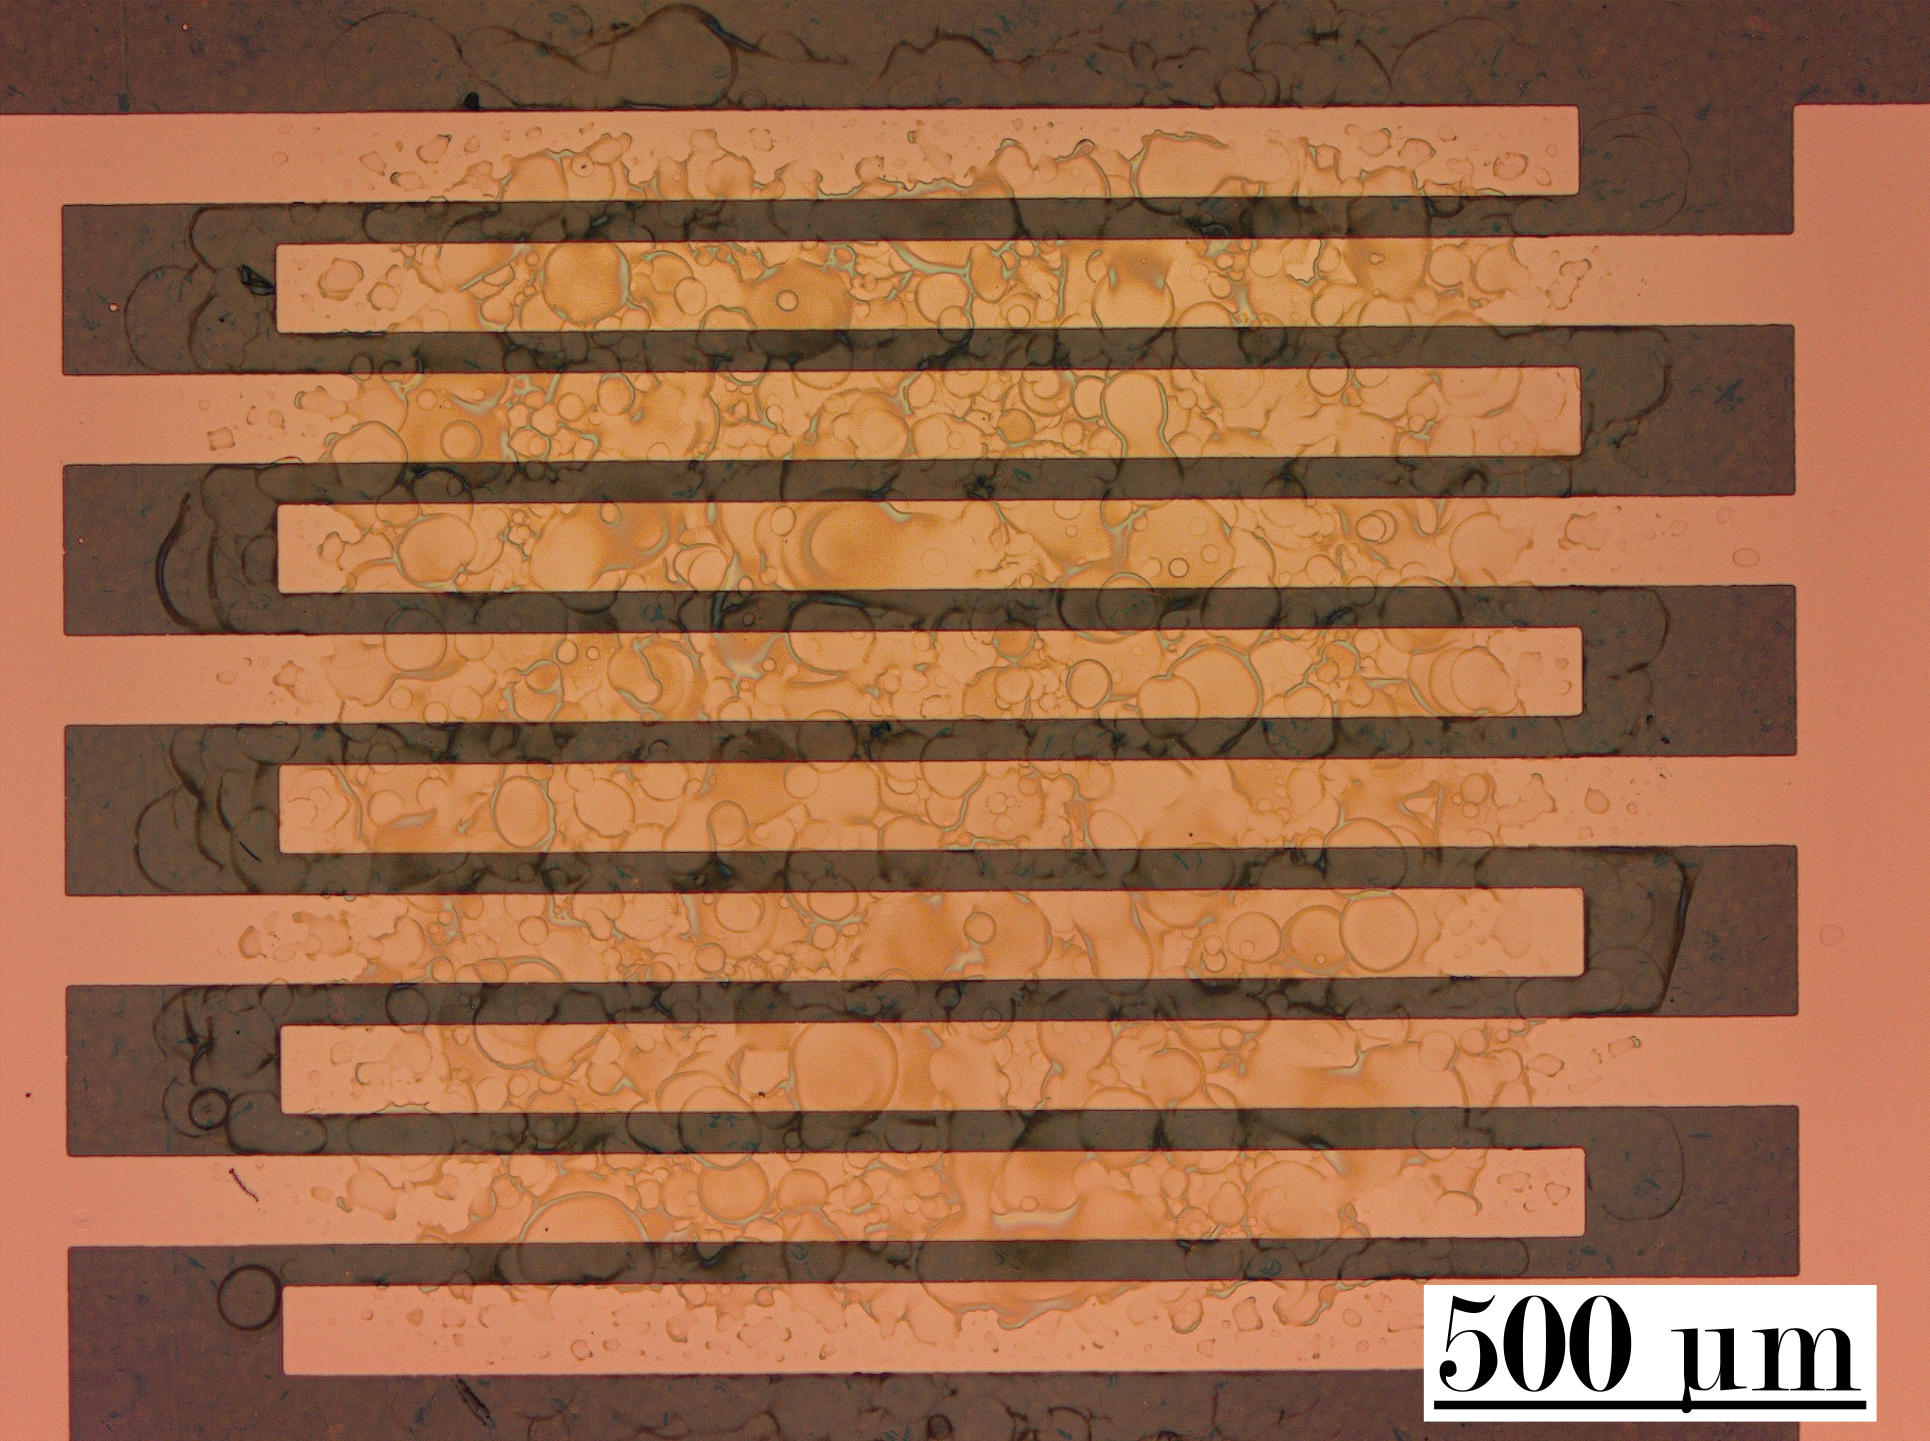
\includegraphics[height=3.3cm]{figures/chapter2/cntDeposition/opticalMicroscopeCNT.png}
        \label{fig:CNTopticalMicroscope}
    }
    \quad
    \subfloat[AFM]{%
        \includegraphics[height=3.3cm]{figures/chapter2/cntDeposition/Fig10_afmCNT.jpg}
        \label{fig:AFM}
    }
    \quad
    \subfloat[SEM]{%
        \includegraphics[height=3.3cm]{figures/chapter2/cntDeposition/semCNT.png}
        \label{fig:SEM}
    }
    \caption{Morphological characterization of the sprayed SWCNTs. (a) With an optical microscope, the SWCNTs are not visible. This is still a valuable tool to predict CNT density during the calibration steps of the process, before surfactant removal. (b, c) After surfactant removal, a uniform random CNT network can be observed in AFM and SEM images. The uniform density and distribution, together with the absence of bundles ensure proper conduction, which is essential for the correct functioning of the fabricated EG-FETs.}
    \label{fig:morphoCNT}
\end{figure}
